% !Mode:: "TeX:UTF-8" 



\BiSection{2.11}{Figures}

\fancyhead[R]{本题2.11由QC.Z完成}

解:

\scalebox{3}{(a)}

当$V_G-V_X<V_{TH}$即$V_X>2.3V$时,NFET关

饱和区$I_D=\frac{1}{2}\mu_nC_{ox}\frac{W}{L}(3V-V_X-0.7V)^2$

$I_D=C_1\frac{dV_X}{dt}$

联立以上两式

$\frac{1}{2}\mu_nC_{ox}\frac{W}{L}(2.3V-V_X)^2(\frac{1}{C_1})=\frac{dV_X}{dt}$

令$\alpha=(\frac{1}{2}\mu_nC_{ox}\frac{W}{L})(\frac{1}{C_1})$

$\alpha (2.3V-V_X)^2=\frac{dV_X}{dt}$

$\alpha \int dt =\int \frac{dV_X}{(2.3V-V_X)^2}$

$\alpha t+k=\frac{1}{2.3V-V_X}$\ding{172}

$(\alpha) (0)+k=\frac{1}{2.3V-1V}$

$k=\frac{1}{1.3V}$

将上式代入\ding{172}

$\alpha t+\frac{1}{1.3V}=\frac{1}{2.3V-V_X}$

$2.3V-V_X=\frac{1}{\alpha t+\frac{1}{1.3V}}$

$V_X=2.3V-\frac{1}{\alpha t+\frac{1}{1.3V}}$

$V_X=2.3V-\frac{1}{(\alpha) (0)+\frac{1}{1.3V}}=1V$

		\begin{figure}[H] %H为当前位置,!htb为忽略美学标准,htbp为浮动图形
	\begin{minipage}{\linewidth}
		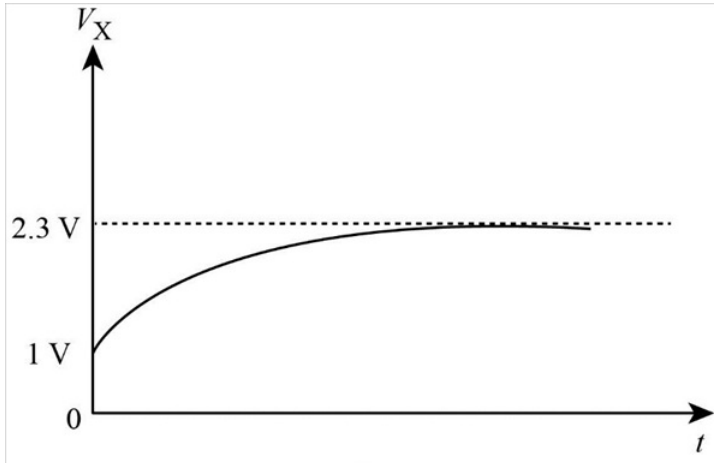
\includegraphics[width=1\linewidth]{2.11-1}
	\end{minipage}
	\caption*{图1} %最终文档中希望显示的图片标题
\end{figure}

\scalebox{3}{(b)}

线性区$I_D=\mu_nC_{ox}\frac{W}{L}[(V_{G}-V_{TH})V_{X}-\frac{1}{2}V_{X}^2]=\mu_nC_{ox}\frac{W}{L}[(3V-0.7V)V_{X}-\frac{1}{2}V_{X}^2]=\mu_nC_{ox}\frac{W}{L}[(2.3V)V_{X}-\frac{1}{2}V_{X}^2]$

$I_D=-C_1\frac{dV_X}{dt}$

联立以上两式

$\mu_nC_{ox}\frac{W}{L}[(2.3V)V_{X}-\frac{1}{2}V_{X}^2]=-C_1\frac{dV_X}{dt}$

$\frac{1}{2}\mu_nC_{ox}\frac{W}{L}(\frac{1}{C_1})[(4.6V)V_{X}-V_{X}^2]=-\frac{dV_X}{dt}$

令$\alpha=(\frac{1}{2}\mu_nC_{ox}\frac{W}{L})(\frac{1}{C_1})$

$\alpha[(4.6V)V_{X}-V_{X}^2]=-\frac{dV_X}{dt}$

	\begin{figure}[H] %H为当前位置,!htb为忽略美学标准,htbp为浮动图形
	\begin{minipage}{\linewidth}
		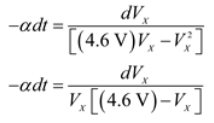
\includegraphics{2.11-2}
	\end{minipage}
\end{figure}

	\begin{figure}[H] %H为当前位置,!htb为忽略美学标准,htbp为浮动图形
	\begin{minipage}{\linewidth}
		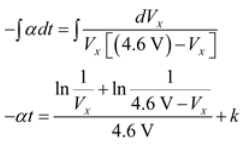
\includegraphics{2.11-3}
	\end{minipage}
\end{figure}

	\begin{figure}[H] %H为当前位置,!htb为忽略美学标准,htbp为浮动图形
	\begin{minipage}{\linewidth}
		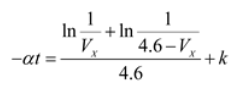
\includegraphics{2.11-4}
	\end{minipage}
\end{figure}

	\begin{figure}[H] %H为当前位置,!htb为忽略美学标准,htbp为浮动图形
	\begin{minipage}{\linewidth}
		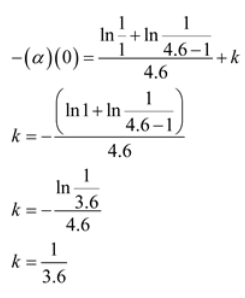
\includegraphics{2.11-5}
	\end{minipage}
\end{figure}

	\begin{figure}[H] %H为当前位置,!htb为忽略美学标准,htbp为浮动图形
	\begin{minipage}{\linewidth}
		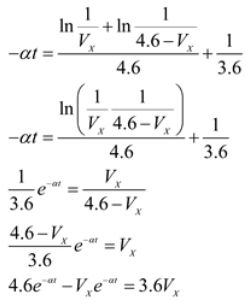
\includegraphics{2.11-6}
	\end{minipage}
\end{figure}

	\begin{figure}[H] %H为当前位置,!htb为忽略美学标准,htbp为浮动图形
	\begin{minipage}{\linewidth}
		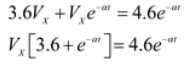
\includegraphics{2.11-7}
	\end{minipage}
\end{figure}

	\begin{figure}[H] %H为当前位置,!htb为忽略美学标准,htbp为浮动图形
	\begin{minipage}{\linewidth}
		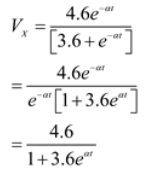
\includegraphics{2.11-8}
	\end{minipage}
\end{figure}



$V_X=\frac{4.6}{1+3.6e^{\alpha (0)}}=1V$

		\begin{figure}[H] %H为当前位置,!htb为忽略美学标准,htbp为浮动图形
	\begin{minipage}{\linewidth}
		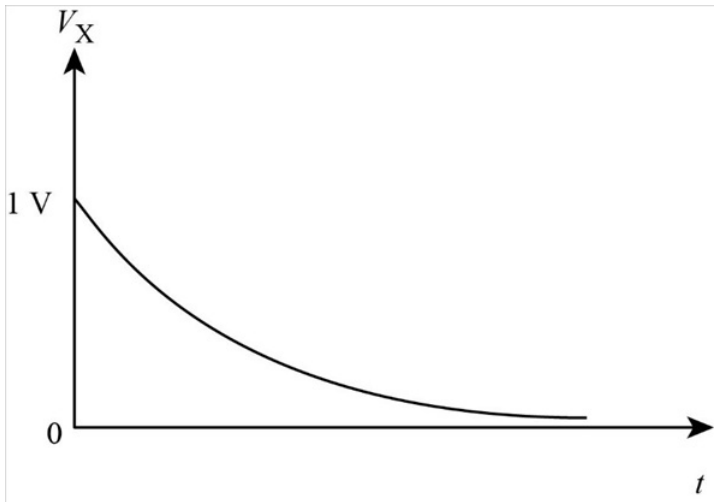
\includegraphics[width=1\linewidth]{2.11-9}
	\end{minipage}
	\caption*{图2} %最终文档中希望显示的图片标题
\end{figure}

\scalebox{3}{(c)}

当$V_{X}>V_{in}-V_{TH}$即$V_{X}>2.3V$($t<t_0$)时,饱和区$I_D=\frac{1}{2}\mu_nC_{ox}\frac{W}{L}(3V-0.7V)^2=\frac{1}{2}\mu_nC_{ox}\frac{W}{L}(2.3V)^2$

$V_X=5V-\frac{I_Dt}{C_1}=5V-\frac{1}{2}\mu_nC_{ox}\frac{W}{L}(2.3V)^2\frac{t}{C_1}$

当$V_{X}<V_{in}-V_{TH}$即$V_{X}<2.3V$($t>t_0$)时,线性区$I_D=\mu_nC_{ox}\frac{W}{L}[(V_{G}-V_{TH})V_{X}-\frac{1}{2}V_{X}^2]=\frac{1}{2}\mu_nC_{ox}\frac{W}{L}[2(V_{G}-V_{TH})V_{X}-V_{X}^2]=\frac{1}{2}\mu_nC_{ox}\frac{W}{L}[2(3V-0.7V)V_{X}-V_{X}^2]=\frac{1}{2}\mu_nC_{ox}\frac{W}{L}[(4.6V)V_{X}-V_{X}^2]$

$I_D=-C_1\frac{dV_X}{dt}$

联立以上二式

	\begin{figure}[H] %H为当前位置,!htb为忽略美学标准,htbp为浮动图形
	\begin{minipage}{\linewidth}
		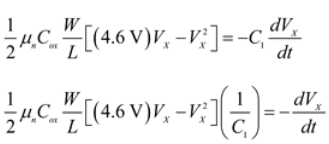
\includegraphics{2.11-10}
	\end{minipage}
\end{figure}


令$\alpha=(\frac{1}{2}\mu_nC_{ox}\frac{W}{L})(\frac{1}{C_1})$

	\begin{figure}[H] %H为当前位置,!htb为忽略美学标准,htbp为浮动图形
	\begin{minipage}{\linewidth}
		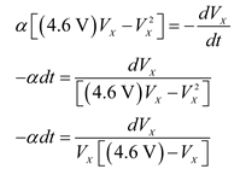
\includegraphics{2.11-11}
	\end{minipage}
\end{figure}

	\begin{figure}[H] %H为当前位置,!htb为忽略美学标准,htbp为浮动图形
	\begin{minipage}{\linewidth}
		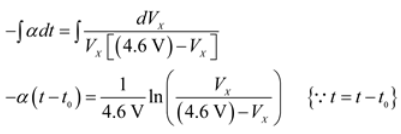
\includegraphics{2.11-12}
	\end{minipage}
\end{figure}

	\begin{figure}[H] %H为当前位置,!htb为忽略美学标准,htbp为浮动图形
	\begin{minipage}{\linewidth}
		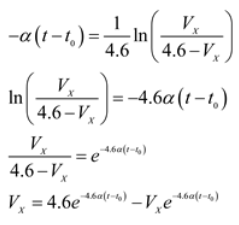
\includegraphics{2.11-13}
	\end{minipage}
\end{figure}

	\begin{figure}[H] %H为当前位置,!htb为忽略美学标准,htbp为浮动图形
	\begin{minipage}{\linewidth}
		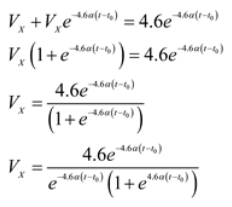
\includegraphics{2.11-14}
	\end{minipage}
\end{figure}



$V_X=\frac{4.6}{1+e^{4.6 \alpha (t-t_0)}}$

		\begin{figure}[H] %H为当前位置,!htb为忽略美学标准,htbp为浮动图形
	\begin{minipage}{\linewidth}
		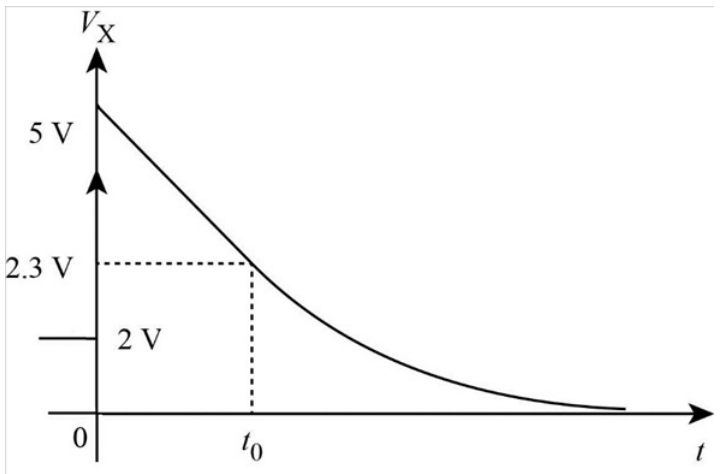
\includegraphics[width=1\linewidth]{2.11-15}
	\end{minipage}
	\caption*{图3} %最终文档中希望显示的图片标题
\end{figure}

\scalebox{3}{(d)}

当$V_{X}>V_{DD}-V_{TH}$即$V_{X}>2.3V$($t<t_0$)时,饱和区$I_D=\frac{1}{2}\mu_nC_{ox}\frac{W}{L}(3V-0.7V)^2=\frac{1}{2}\mu_nC_{ox}\frac{W}{L}(2.3V)^2$

$V_X=3V-\frac{I_Dt}{C_1}=3V-\frac{1}{2}\mu_nC_{ox}\frac{W}{L}(2.3V)^2\frac{t}{C_1}$

当$V_{X}<V_{DD}-V_{TH}$即$V_{X}<2.3V$($t>t_0$)时,线性区$I_D=\frac{1}{2}\mu_nC_{ox}\frac{W}{L}[2(V_{G}-V_{TH})V_{X}-V_{X}^2]=\frac{1}{2}\mu_nC_{ox}\frac{W}{L}[2(3V-0.7V)V_{X}-V_{X}^2]=\frac{1}{2}\mu_nC_{ox}\frac{W}{L}[(4.6V)V_{X}-V_{X}^2]$

$I_D=-C_1\frac{dV_X}{dt}$

联立以上二式

\begin{figure}[H] %H为当前位置,!htb为忽略美学标准,htbp为浮动图形
	\begin{minipage}{\linewidth}
		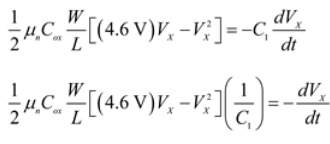
\includegraphics{2.11-16}
	\end{minipage}
\end{figure}

令$\alpha=(\frac{1}{2}\mu_nC_{ox}\frac{W}{L})(\frac{1}{C_1})$

\begin{figure}[H] %H为当前位置,!htb为忽略美学标准,htbp为浮动图形
	\begin{minipage}{\linewidth}
		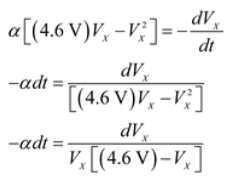
\includegraphics{2.11-17}
	\end{minipage}
\end{figure}

\begin{figure}[H] %H为当前位置,!htb为忽略美学标准,htbp为浮动图形
	\begin{minipage}{\linewidth}
		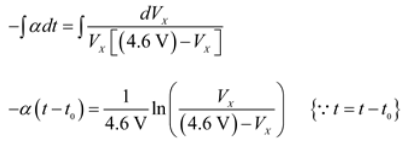
\includegraphics{2.11-18}
	\end{minipage}
\end{figure}

\begin{figure}[H] %H为当前位置,!htb为忽略美学标准,htbp为浮动图形
	\begin{minipage}{\linewidth}
		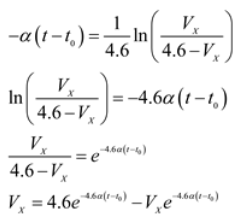
\includegraphics{2.11-19}
	\end{minipage}
\end{figure}

\begin{figure}[H] %H为当前位置,!htb为忽略美学标准,htbp为浮动图形
	\begin{minipage}{\linewidth}
		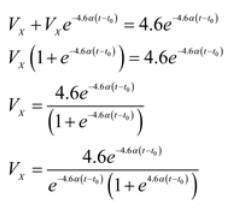
\includegraphics{2.11-20}
	\end{minipage}
\end{figure}


$V_X=\frac{4.6}{1+e^{4.6 \alpha (t-t_0)}}$

\begin{figure}[H] %H为当前位置,!htb为忽略美学标准,htbp为浮动图形
	\begin{minipage}{\linewidth}
		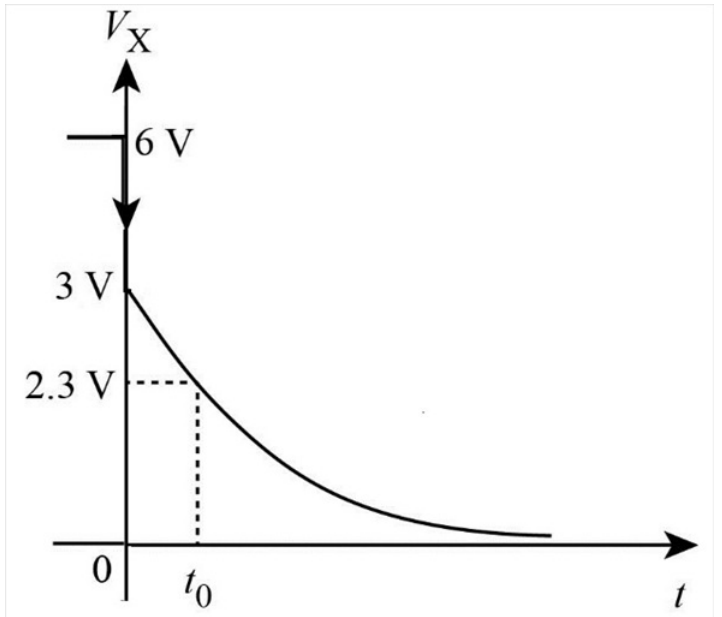
\includegraphics[width=1\linewidth]{2.11-21}
	\end{minipage}
	\caption*{图4} %最终文档中希望显示的图片标题
\end{figure}